\subsection{Optimizer Details (with Hyperparameter values)}\label{subsec:optimizer-details}
In the course of testing these 3 optimizers, we have looked to vary the following hyperparameters: Batch Size, Learning Rate, and Epsilon. We used a basic grid search
approach to testing the hyperparameters for each optimizer. We varied Batch Size from 64 to 1024, we varied learning rate from 0.1 to 0.5, and we varied epsilon from 3 to 50. The
table below shows the entire grid of possible combinations used for each optimizer. The grid search approach allowed us to effectively test the hyperparameter space and appropriately
isolate the effects of these changes. The results of these tests will be provided in the following section.

\begin{table}[h]
    \centering
    \caption{Hyperparameter Grid Search}
    \begin{tabular}{@{}ll@{}}
        \toprule
        \textbf{Hyperparameter}       & \textbf{Values}                           \\ \midrule
        Epsilon                       & [3, 10, 50]                              \\
        Learning Rate                 & [0.1, 0.2, 0.3, 0.4, 0.5]               \\
        Batch Size                    & [64, 128, 256, 512, 1024]                \\
        Noise Multiplier              & 1.1                                       \\
        Epochs                        & 30                                        \\
        Clipping Constant             & 1.0                                       \\ \bottomrule
    \end{tabular}
    \label{tab:hyperparameters}
\end{table}
\break

\subsection{Results varying Learning Rate}\label{subsec:dp-details}
The following results illustrate our current accuracies when varying learning rate for DP-SGD and DP-Adam. We
do not include the current results for DP-RMSProp because we were unable to produce consistent results with while 
varying learning rate. We've seen some evidence, in our testing, that DP-RMSProp should use learning rates that are lower
than those currently tested for the other two optimzers. Results generally show that larger learning rates are bad
for these DP algorithms.

\begin{figure}[ht]
    \centering
    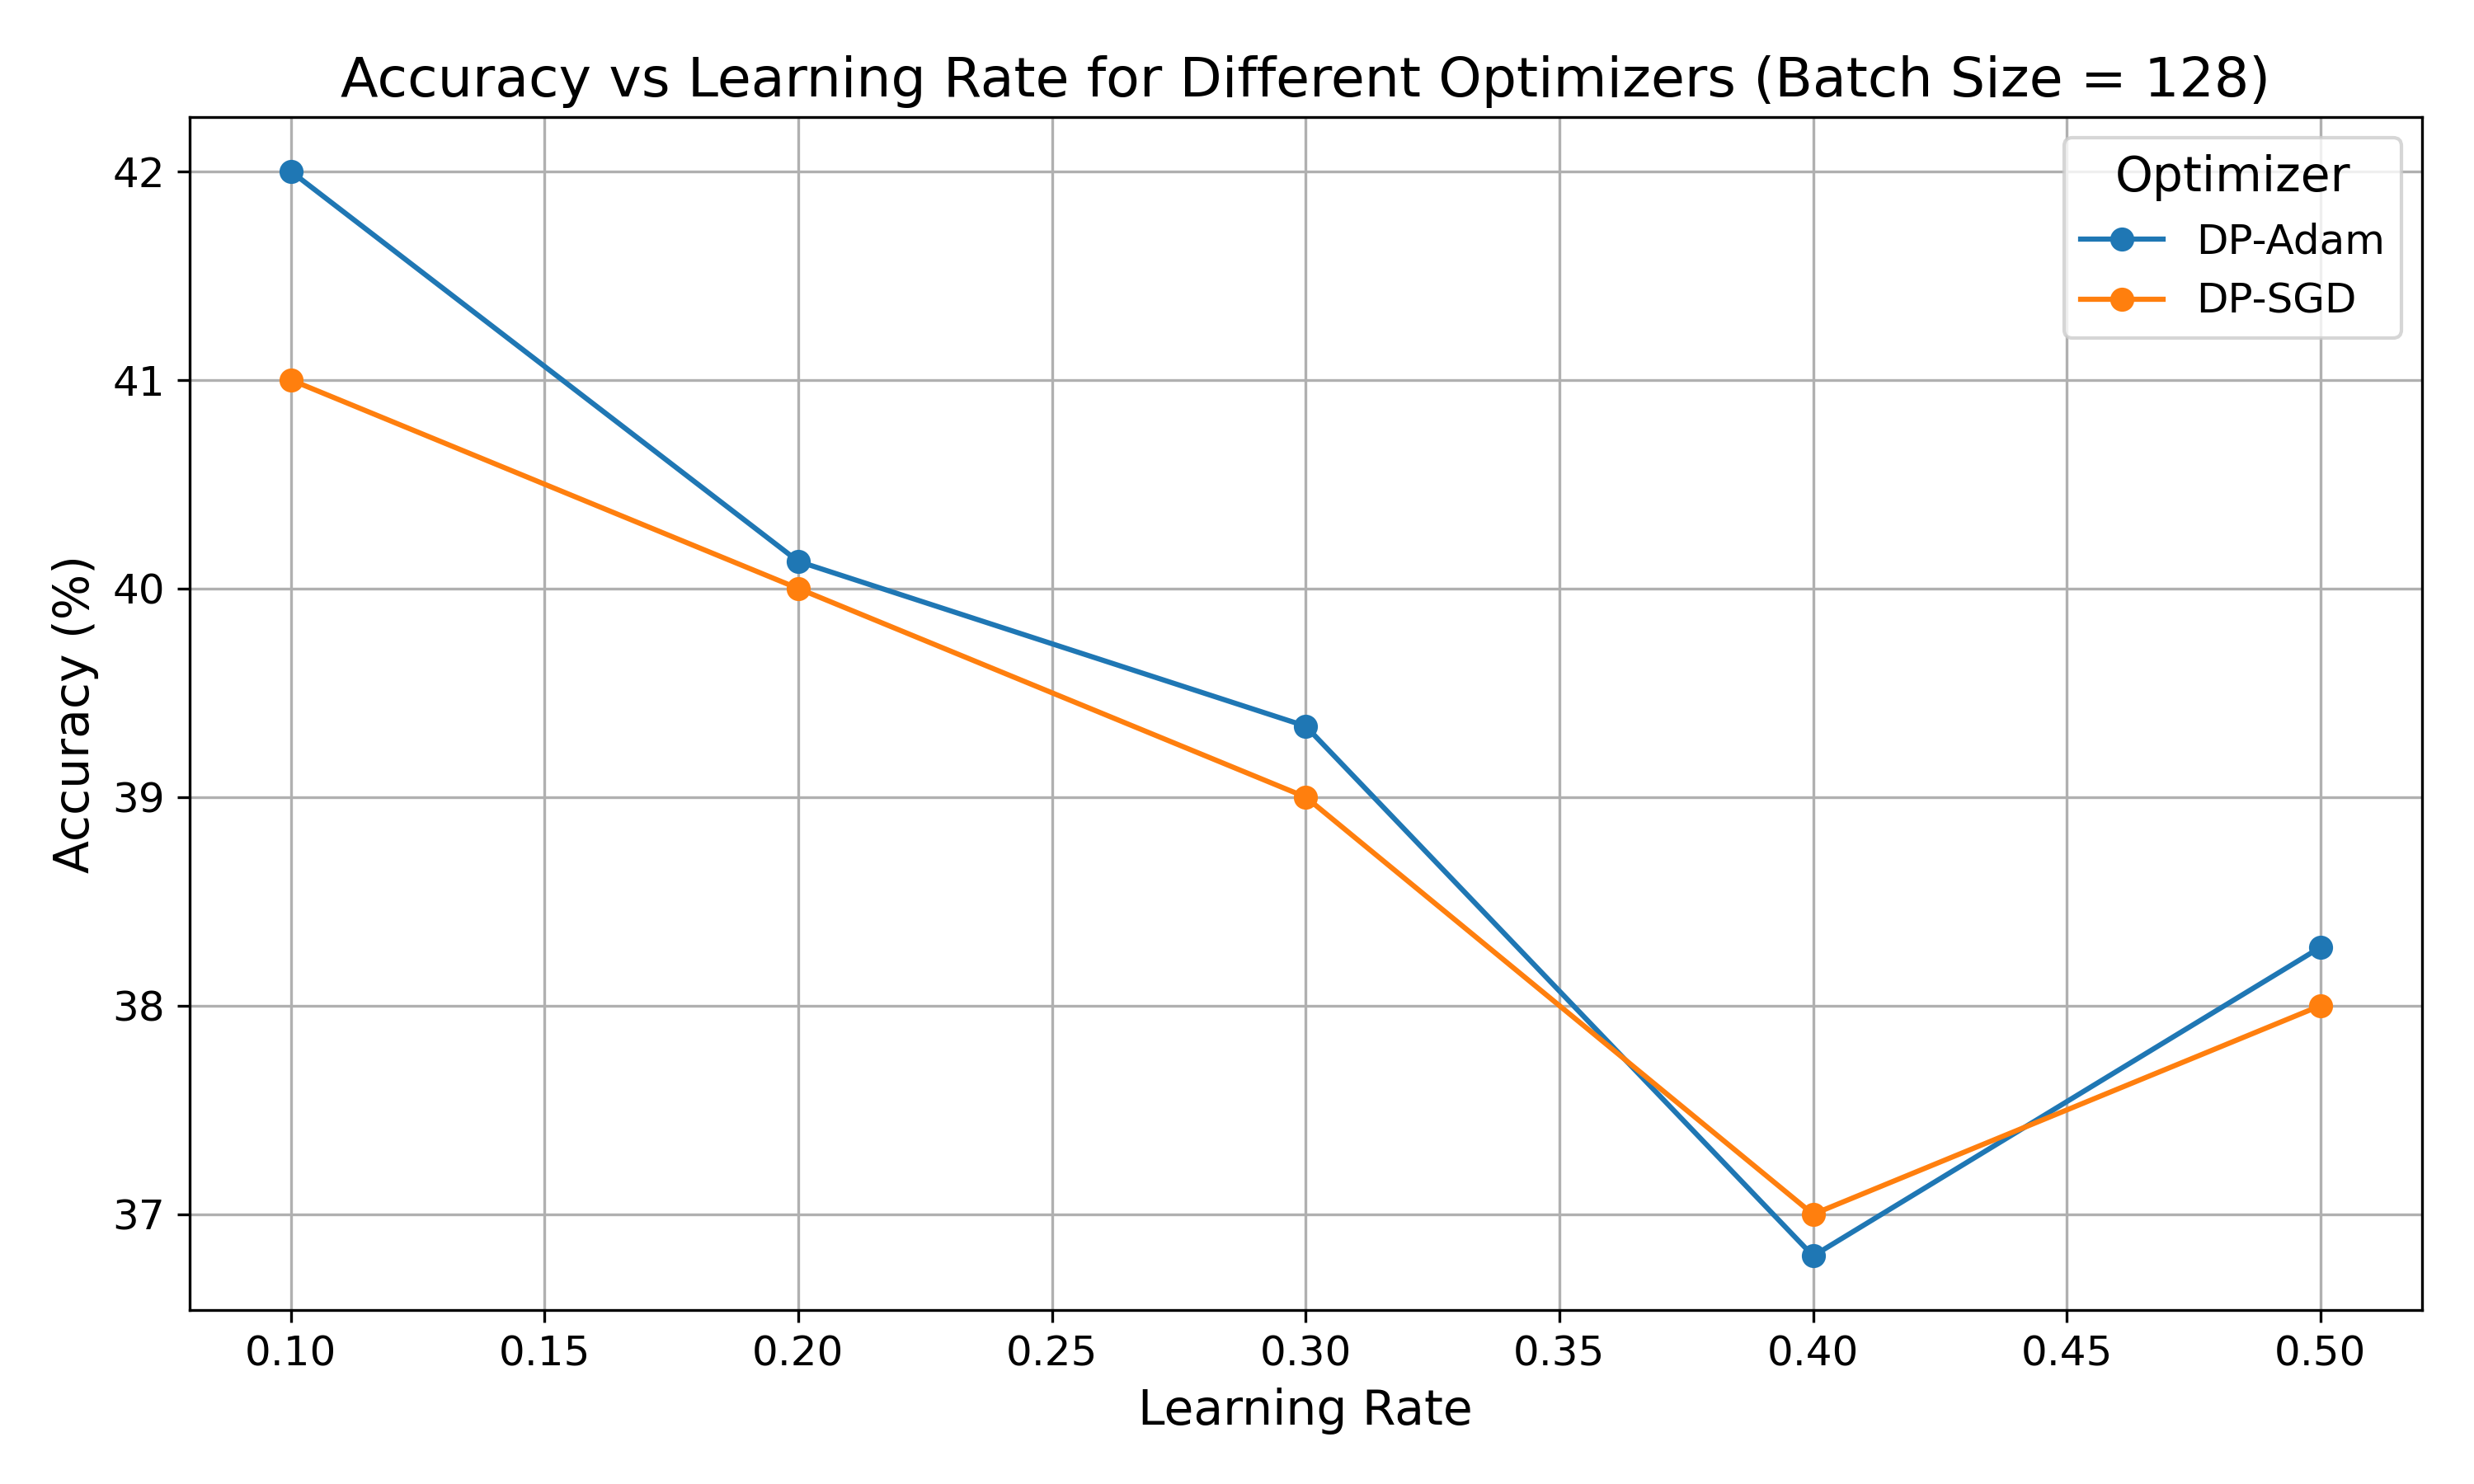
\includegraphics[width=0.65\textwidth]{accuracy_vs_learning_rate.png}
    \caption{Varying Learning Rate for CIFAR-10}
    \label{fig:image_label}
\end{figure}


\subsection{Results varying Batch Size}\label{subsec:dp-details}
The following results illustrate our current accuracies when varying batch size for DP-SGD, DP-RMSProp, and DP-Adam. Accuracy
appears to "cap out" around mid sized batches. Specifically, 256 and 512 appear to provide the greatest utility for our optimizers.
\begin{figure}[ht]
    \centering
    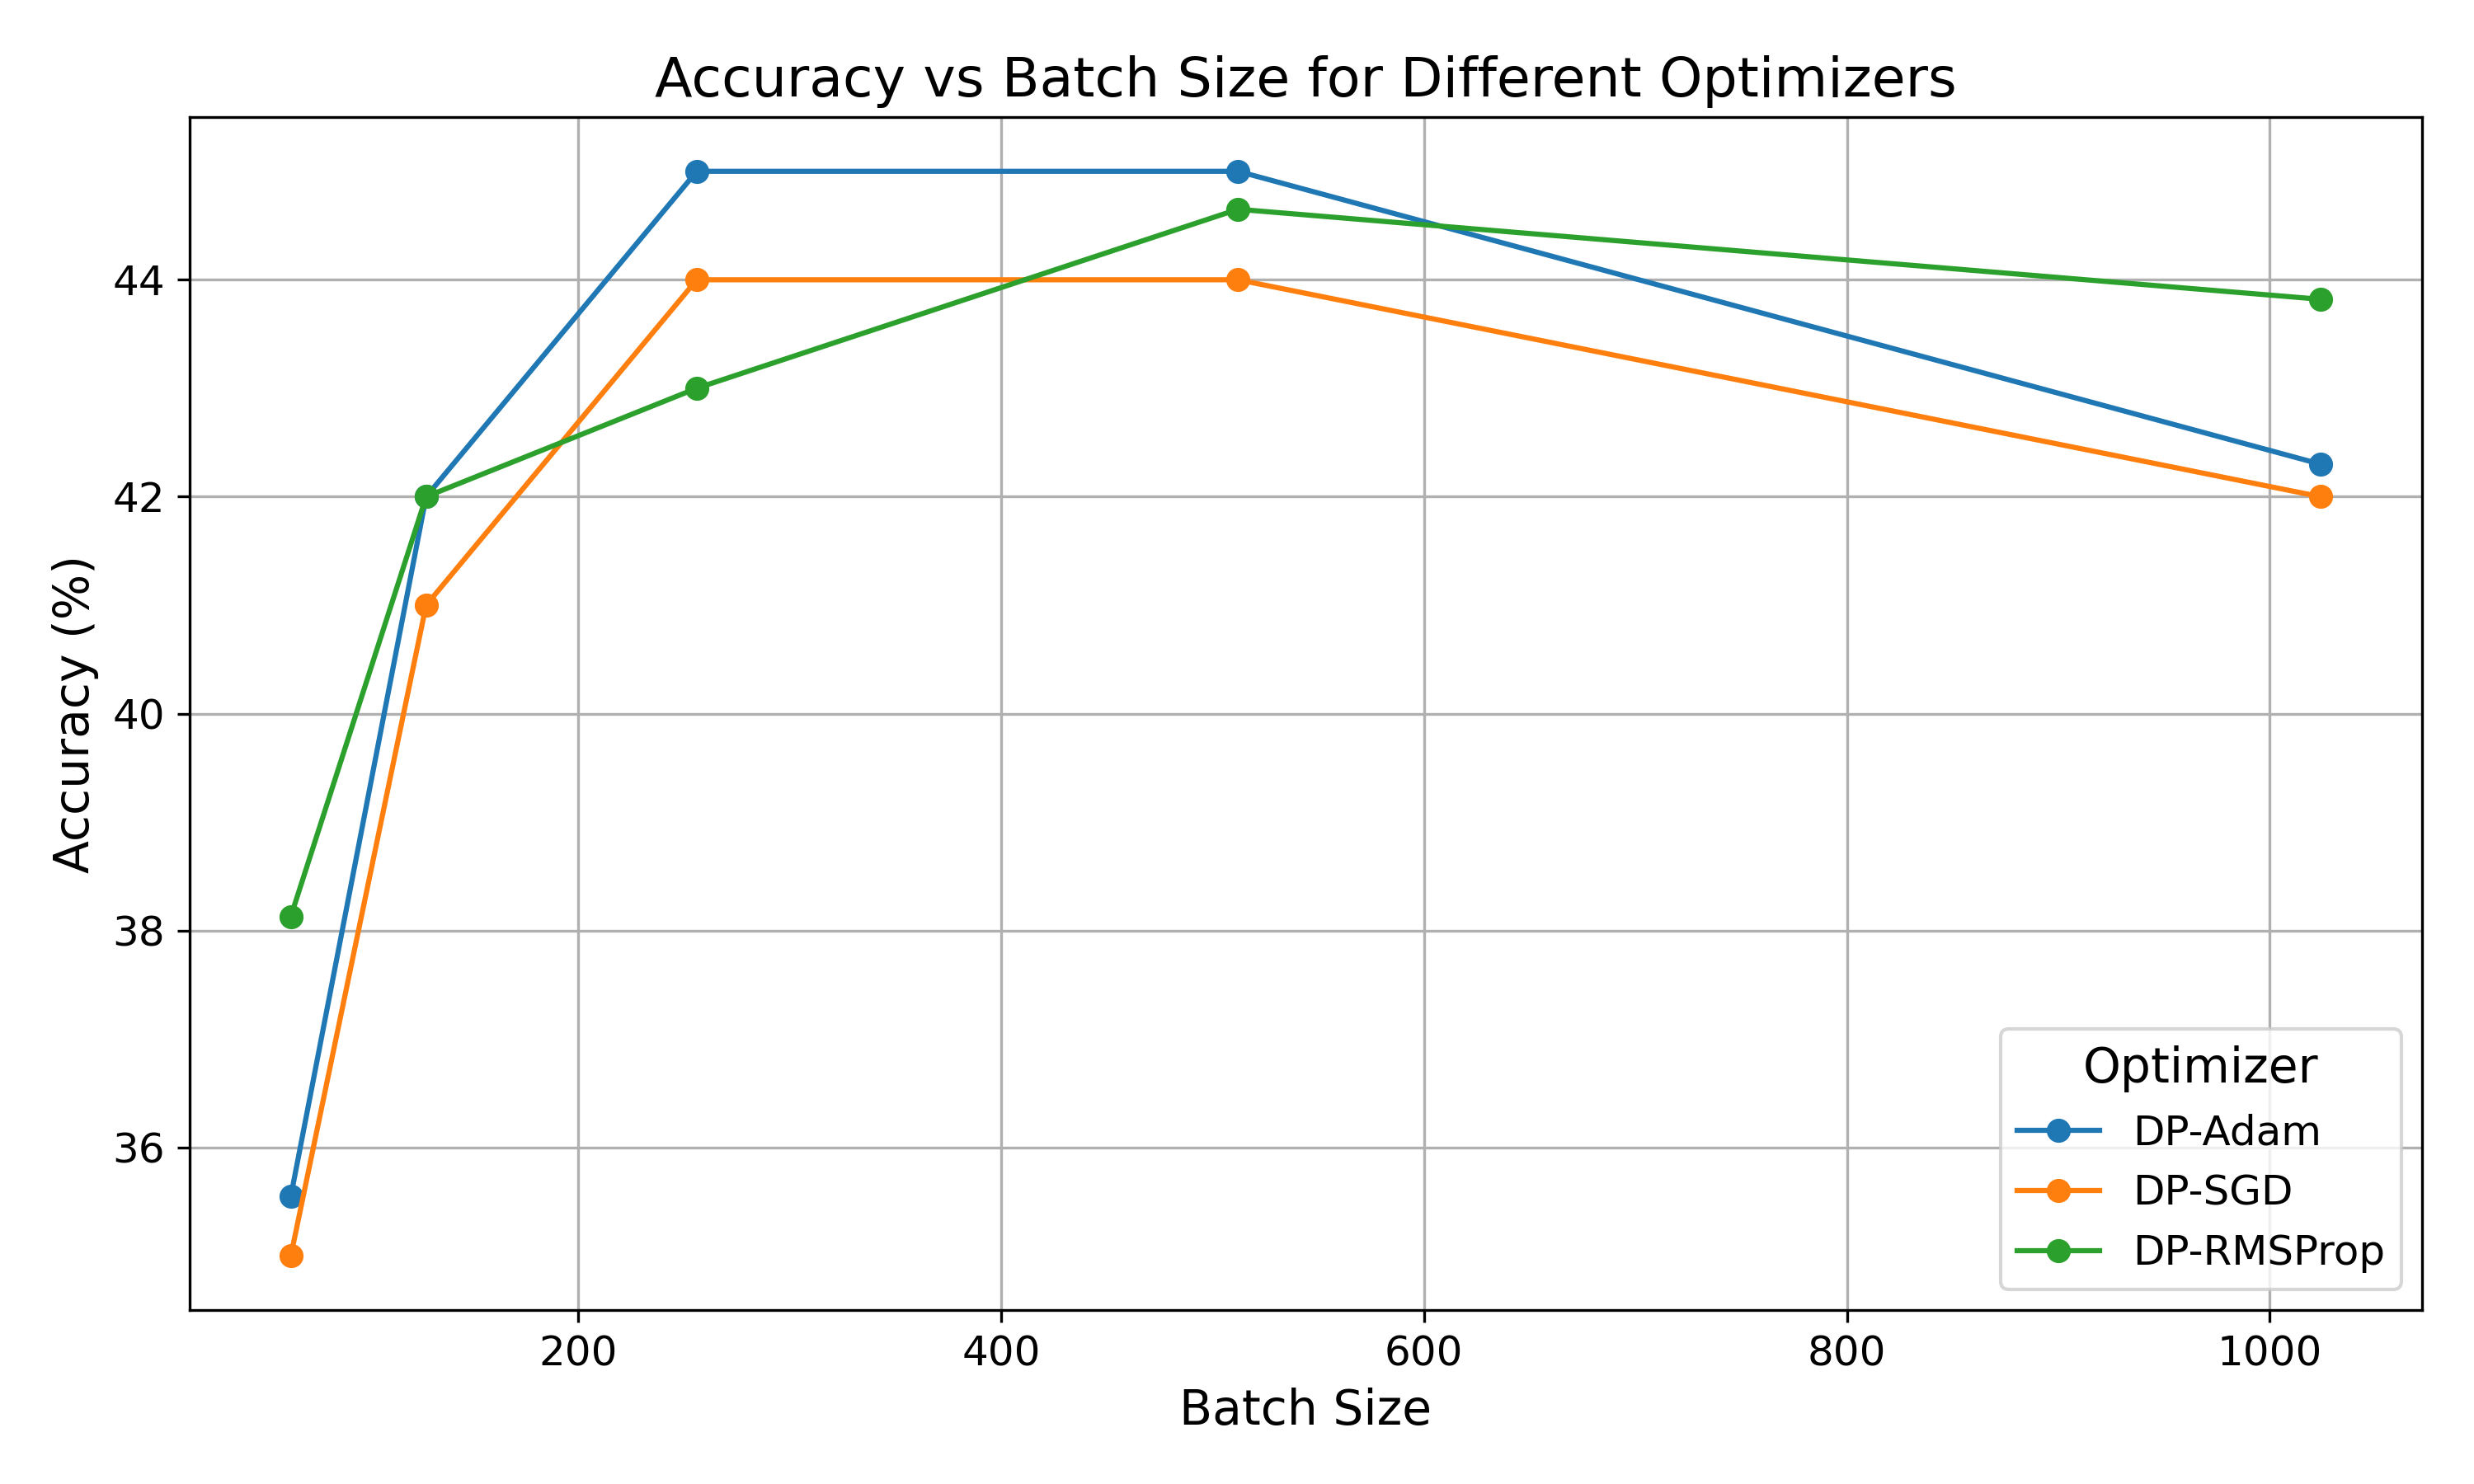
\includegraphics[width=0.65\textwidth]{accuracy_vs_batch_size.png}
    \caption{Varying Batch Size for CIFAR-10}
    \label{fig:image_label}
\end{figure}

\subsection{Results varying Privacy Cost}\label{subsec:dp-details}
The following results illustrate our current accuracies when varying Privacy Budget for DP-SGD, DP-RMSProp, and DP-Adam. For the most
part, accuracies increase as the privacy budget increases. This makes sense as the amount of noise added to the gradients is inversely 
related to the size of the privacy budget (larger $\epsilon$ means lower $\mathcal{N}$). We have an outlier for DP-Adam where the accuracy
is much higher at lower privacy budgets. This will be a point of testing going forward, to determine if this was a statistical anamoly or something
else entirely.

\begin{figure}[ht]
    \centering
    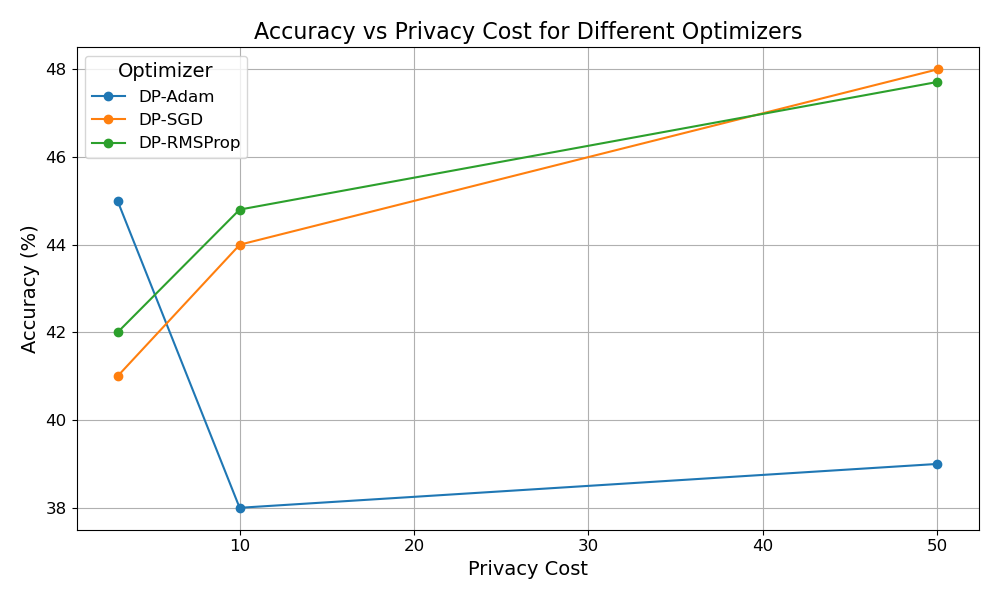
\includegraphics[width=0.65\textwidth]{accuracy_vs_privacy_cost.png}
    \caption{Varying Privacy Cost for CIFAR-10}
    \label{fig:image_label}
\end{figure}

